\subsection{Dice }
I denne klasse bliver der slået med terningerne.
\begin{figure}[H]
    \centering
    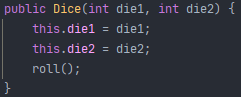
\includegraphics[width=0.7\textwidth]{sources/7_implementering/Dice.PNG}
    \caption{Dice konstruktør}
    \label{fig:DiceKons}
\end{figure}
Dice klassen begyndder med, at vi opretter to die og kalder en roll metode på dem.
\begin{figure}[H]
    \centering
    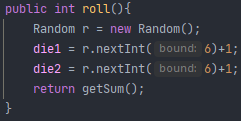
\includegraphics[width=0.7\textwidth]{sources/7_implementering/Roll.PNG}
    \caption{Roll metoden i Dice}
    \label{fig:diceRoll}
\end{figure}
Roll metoden bruger Random metoden, så når terningerne ‘kastes’ vil de hver have en værdi mellem 1 og 6. Der vil ligeledes blive returneret en sum af de to terningers værdier.
\begin{figure}[H]
    \centering
    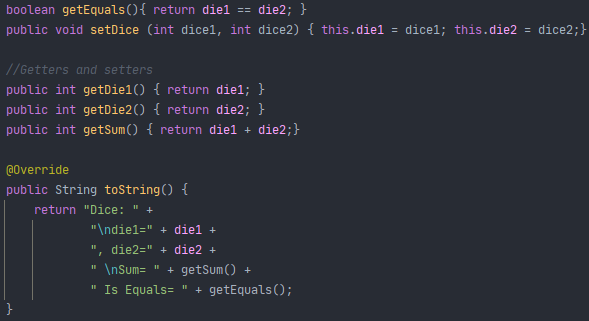
\includegraphics[width=0.7\textwidth]{sources/7_implementering/equal.PNG}
    \caption{Getter og setters, samt toString metode}
    \label{fig:Dicemisc}
\end{figure}
Boolean'en getEquals metoden, viser, når vores terninger har samme værdi, da det resulterer i et ekstra kast.
Herefter har vi først en setDice metode, som bruges til at tilvige terningerne en bestemt værdi, og efterfølgende en getDice metode, som kan returnere udfaldet af de to terninger hver især eller deres sum.
